\newpage
\subsection*{c)}
To start the exercise, we consider the amount of necessary samples used as burn-in, which we set to $N = 100,000$ samples. The following figure shows the draws of $\boldsymbol{t}$ for $d=2$, i.e. one breakpoint.

\begin{figure}[H]
\centering
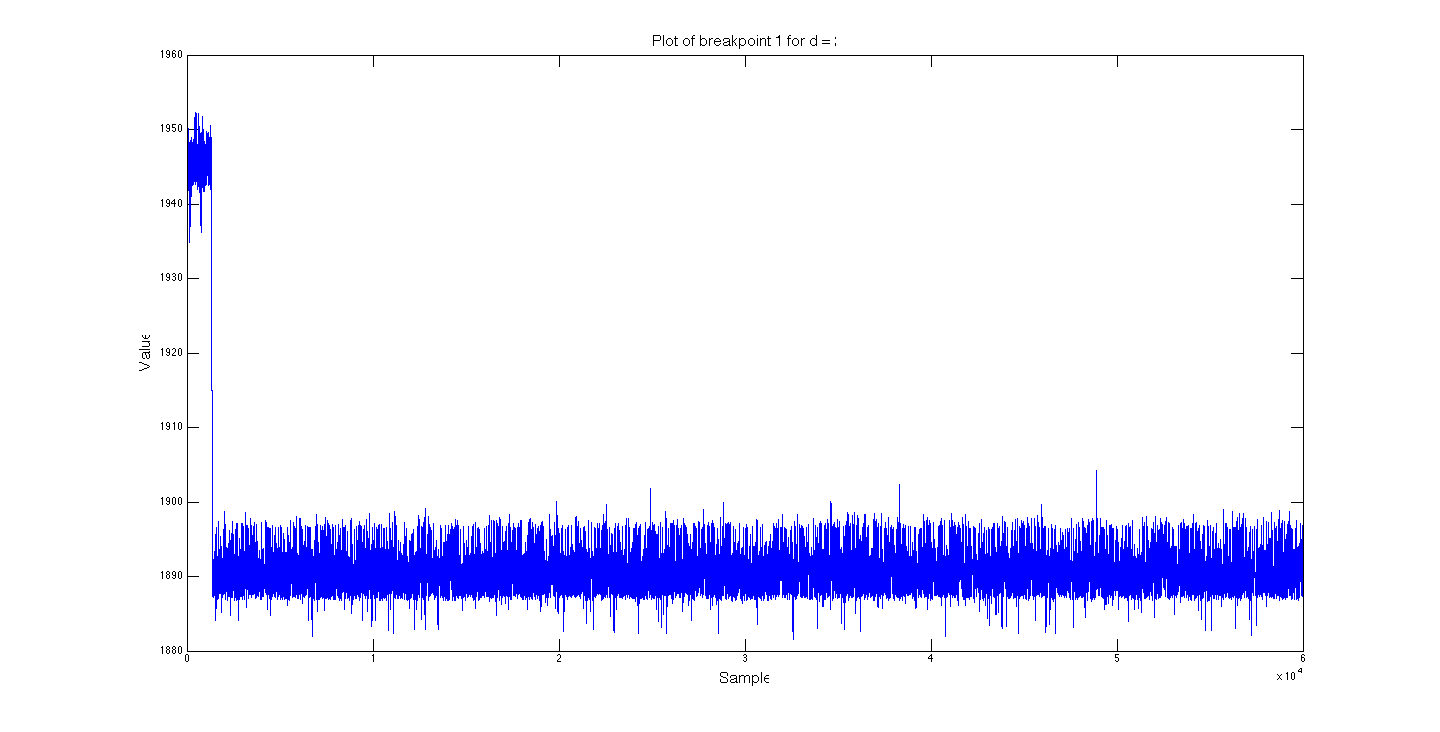
\includegraphics[scale=0.26]{./Figures/iburn.png}
\caption{Figure of the draws of $\boldsymbol{t}$}
\label{fig:burnin}
\end{figure}

As the figures shows, we have stationarity after about $M=3,000$ samples, meaning that our burn-in is reasonable. 

Here in assignment \textbf{c)} we investigate the behaviour of the chain for our posterior $f(\theta,\boldsymbol{\lambda},\boldsymbol{t}|\boldsymbol{\tau})$ for $1,2,3$ and 4 breakpoints in the data. We will show that the posterior of $\boldsymbol{t}$ for the intervals will be affected in various ways depending on the density for each interval.\\

For the remainder of this assignment, we analyze the number of breakpoints individually with $\beta = 1$ and $\rho = (0.05,\:,0.14,\:0.25,\:0.36)$.\\

\newpage
\subsubsection*{One Breakpoint}
If we divide the time period into two intervals we get that the breakpoint is located at $t\approx 1891$. Figure \ref{fig:bp1} shows where the location of the breakpoint is located relative to the dataset in order to get a better overview.

\begin{figure}[H]
\centering
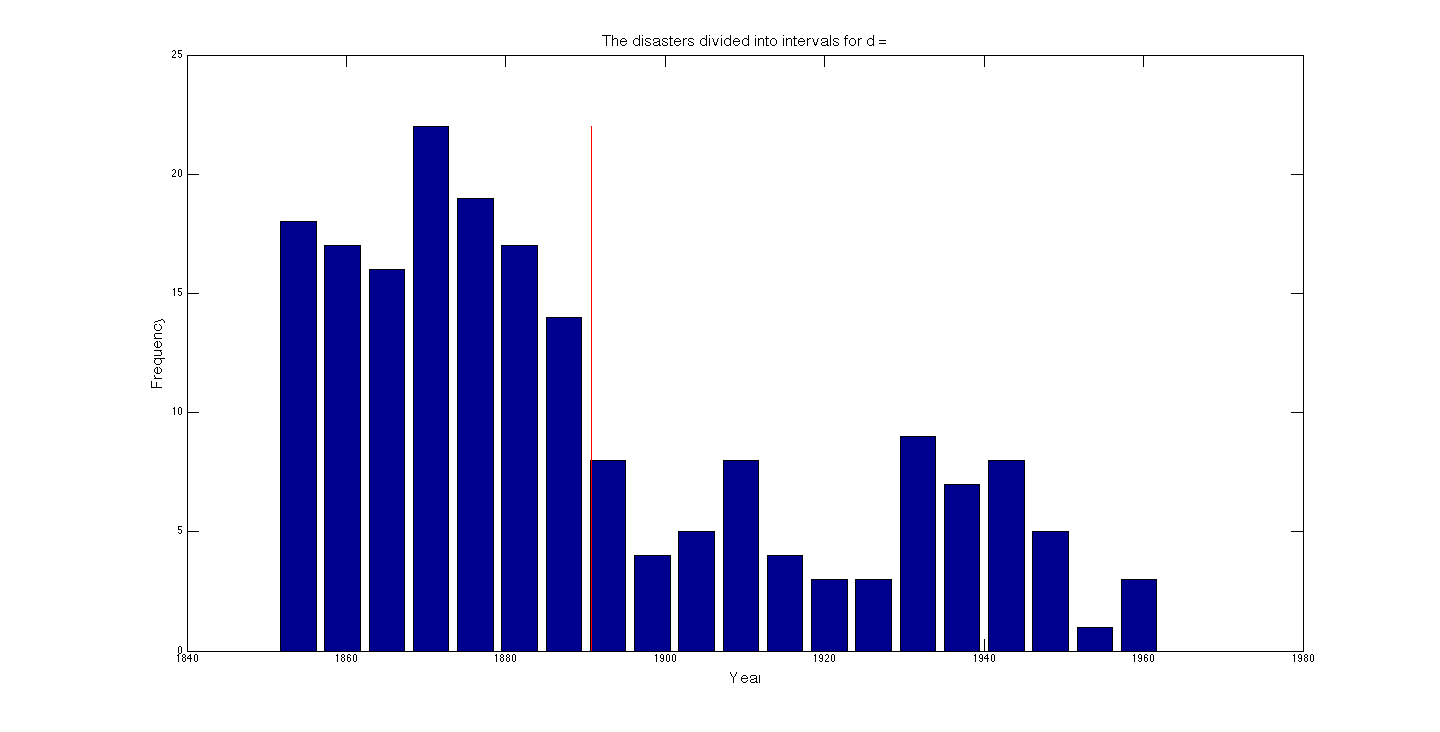
\includegraphics[scale=0.26]{./Figures/bp1.png}
\caption{Plot of where the breakpoint is located.}
\label{fig:bp1}
\end{figure}

In the introduction we said that the breakpoint should lie somewhere at the turn of the century, and as is seen in figure \ref{fig:bp1} we have a reasonable result as to where the breakpoint lies. \\ We now look at the histogram of the breakpoint in figure \ref{fig:tpost1}.

\begin{figure}[H]
\centering
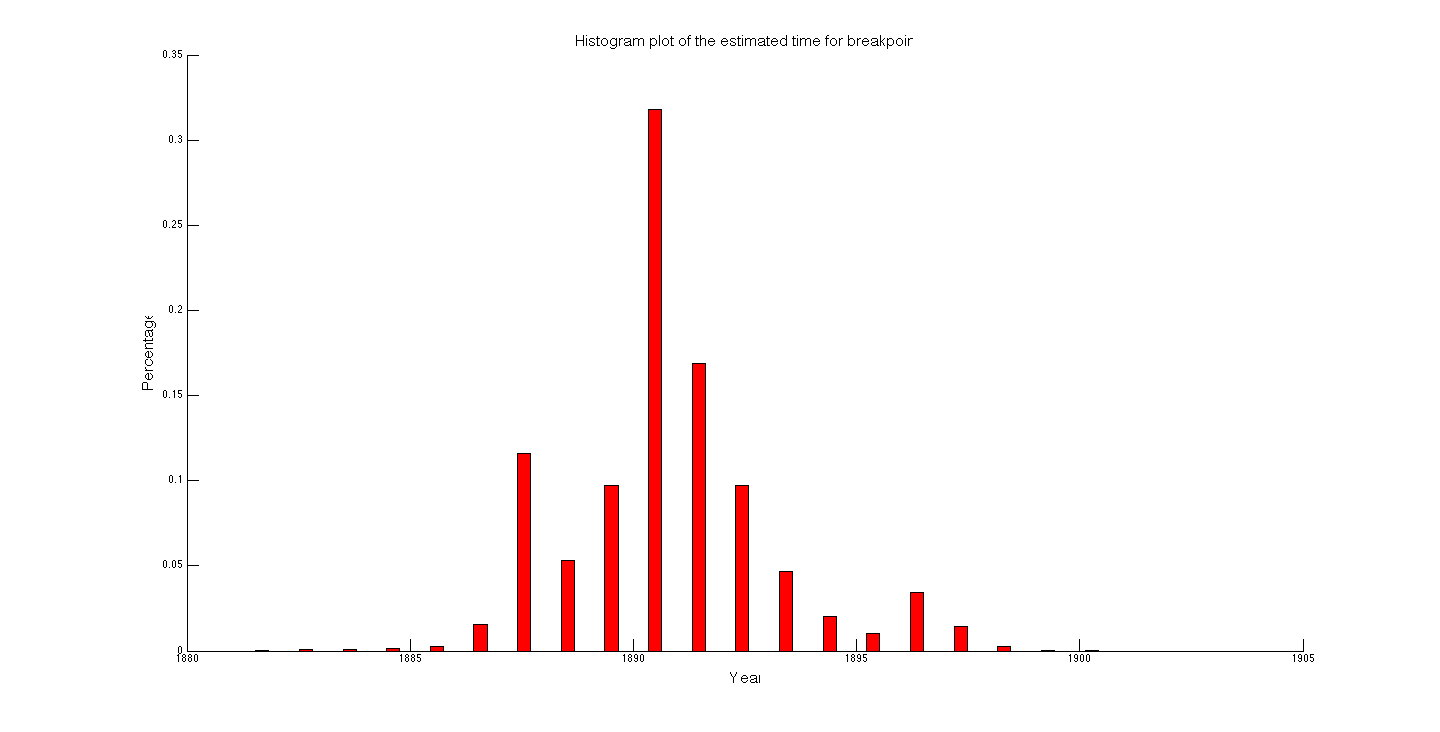
\includegraphics[scale=0.26]{./Figures/tpost1.png}
\caption{Histogram plot of the breakpoint.}
\label{fig:tpost1}
\end{figure}

As is seen in figure \ref{fig:tpost1}, the histogram is centered around 1891 with a small tail indicating a high accuracy in the estimation of the breakpoint. We visualize the draws from the posterior in figure \ref{fig:t1}.

\begin{figure}[H]
\centering
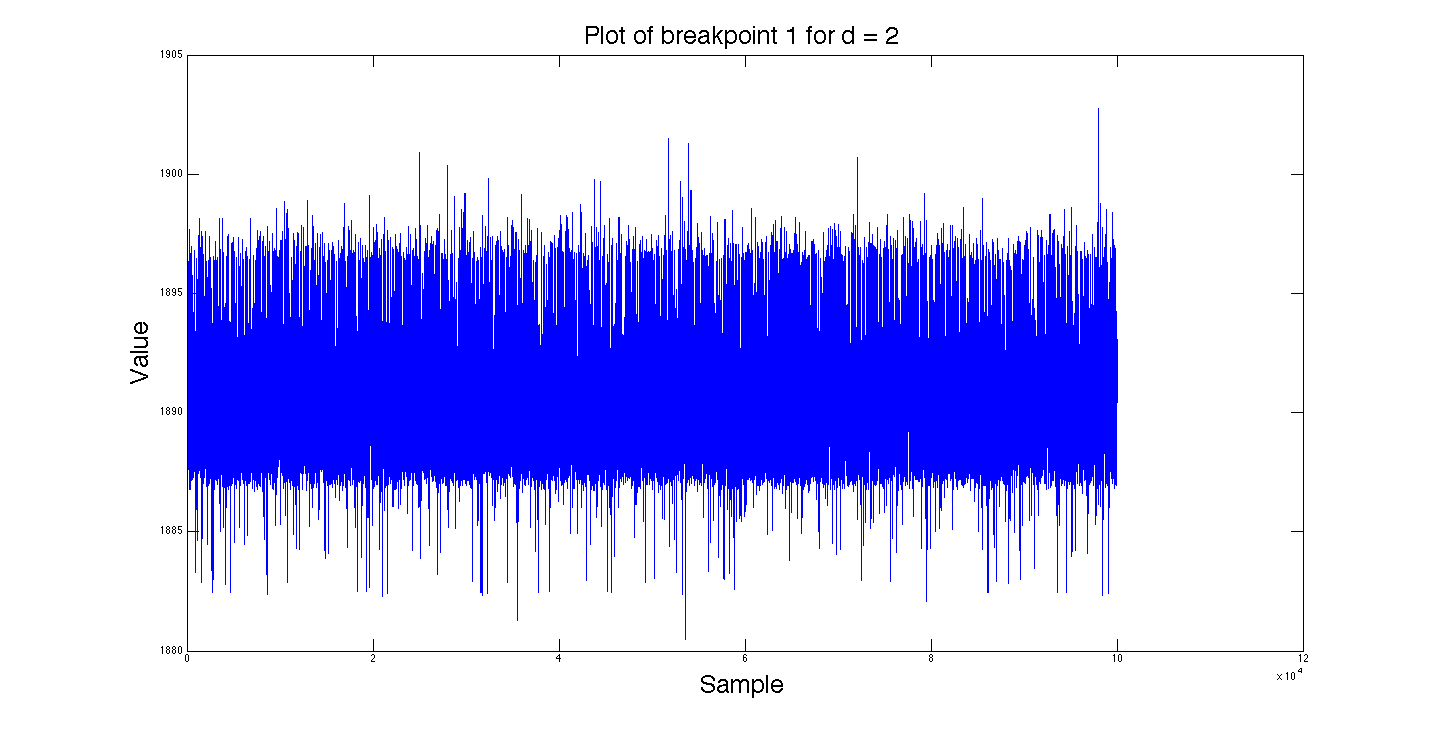
\includegraphics[scale=0.26]{./Figures/t1.png}
\caption{Visualization of the draws for the first breakpoint.}
\label{fig:t1}
\end{figure}

As is seen in the above figure the draws seem to be rather random and not depending on previous values.
We move on to investigate the behaviour of the intensities and see figure \ref{fig:lpost1}.

\begin{figure}[H]
\centering
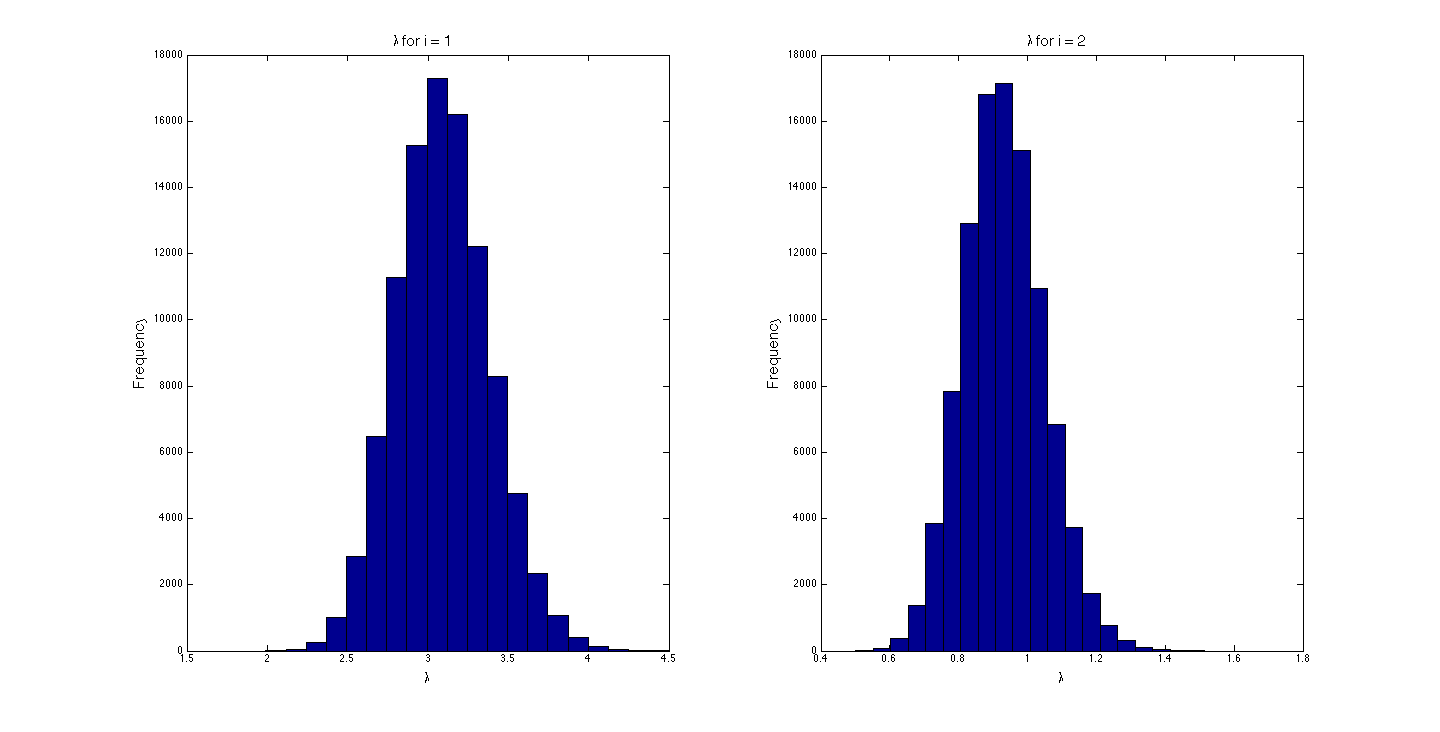
\includegraphics[scale=0.26]{./Figures/lpost1.png}
\caption{Histogram of the intensites of the two intervals.}
\label{fig:lpost1}
\end{figure}

The above figure suggests that the intensites both have a $\Gamma$--distribution where the first intensity is centered around $\approx 3.1$ disasters/year whereas the second intensity is centered around $\approx 0.91$ disasters/year, indicating a decrease of almost 70\%. \\ Finally we look at the histogram of $\theta$, which is seen in figure \ref{fig:thetapost1}.

\begin{figure}[H]
\centering
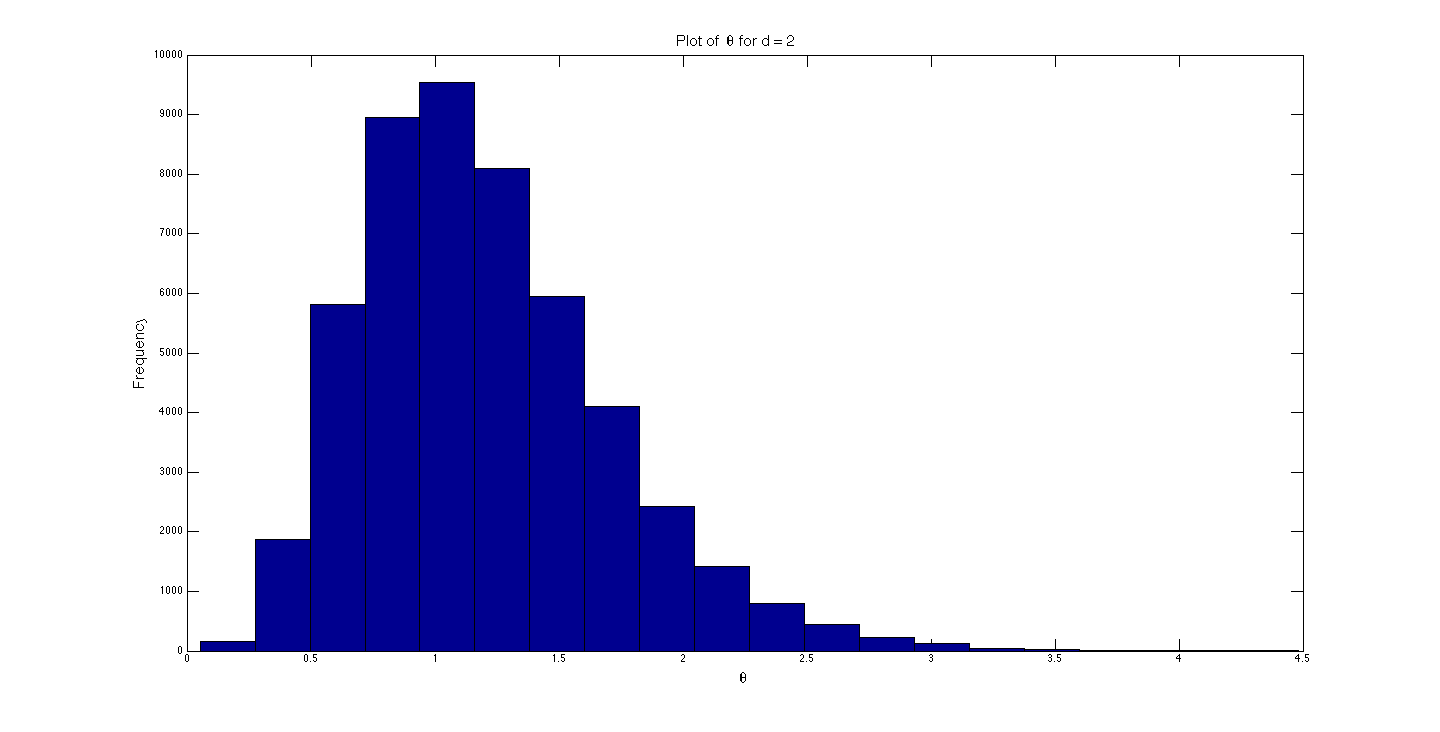
\includegraphics[scale=0.26]{./Figures/thetapost.png}
\caption{Histogram plot of $\theta$.}
\label{fig:thetapost1}
\end{figure}

Figure \ref{fig:thetapost1} is suggestive of a $\Gamma$--distribution centered around $\approx 1.2$. 

\subsubsection*{Two Breakpoints}

We now move on to investigate the behaviour of the chain for two breakpoints. As before, we begin by looking at the location of the breakpoints, which is seen in figure \ref{fig:bp2}.

\begin{figure}[H]
\centering
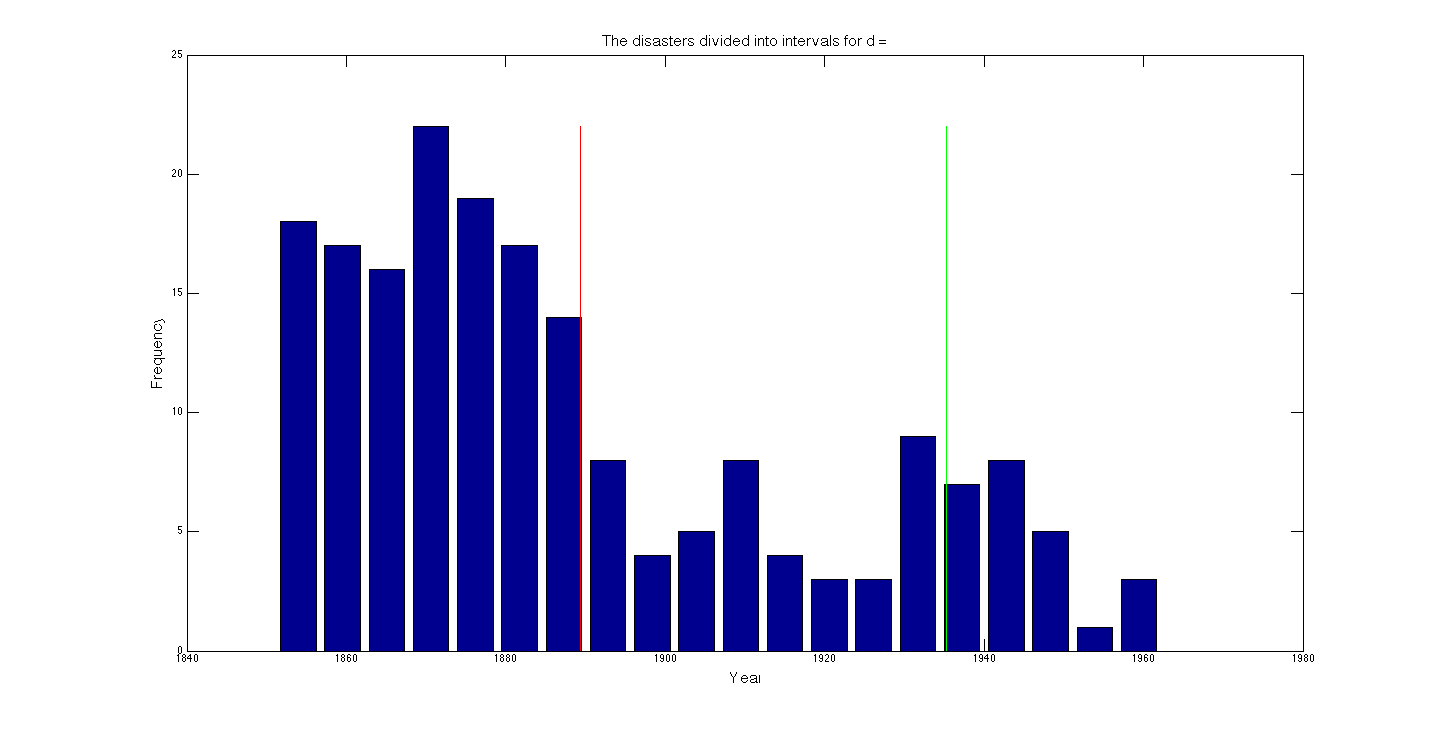
\includegraphics[scale=0.26]{./Figures/bp2.png}
\caption{Plot of where the breakpoints are located.}
\label{fig:bp2}
\end{figure}

As is seen in the above figure, the first breakpoint is almost located at the same time as before. This time it is $\approx 1890$ and the second breakpoint is located at $\approx 1937$. By looking at the figure, a more natural placement of the second breakpoint should be somewhere around 1930 since the change in intensity seems to occur there rather than at 1937. We move on to investigate the behaviour of the histogram of the breakpoints and look at figure \ref{fig:tpost2}.

\begin{figure}[H]
\centering
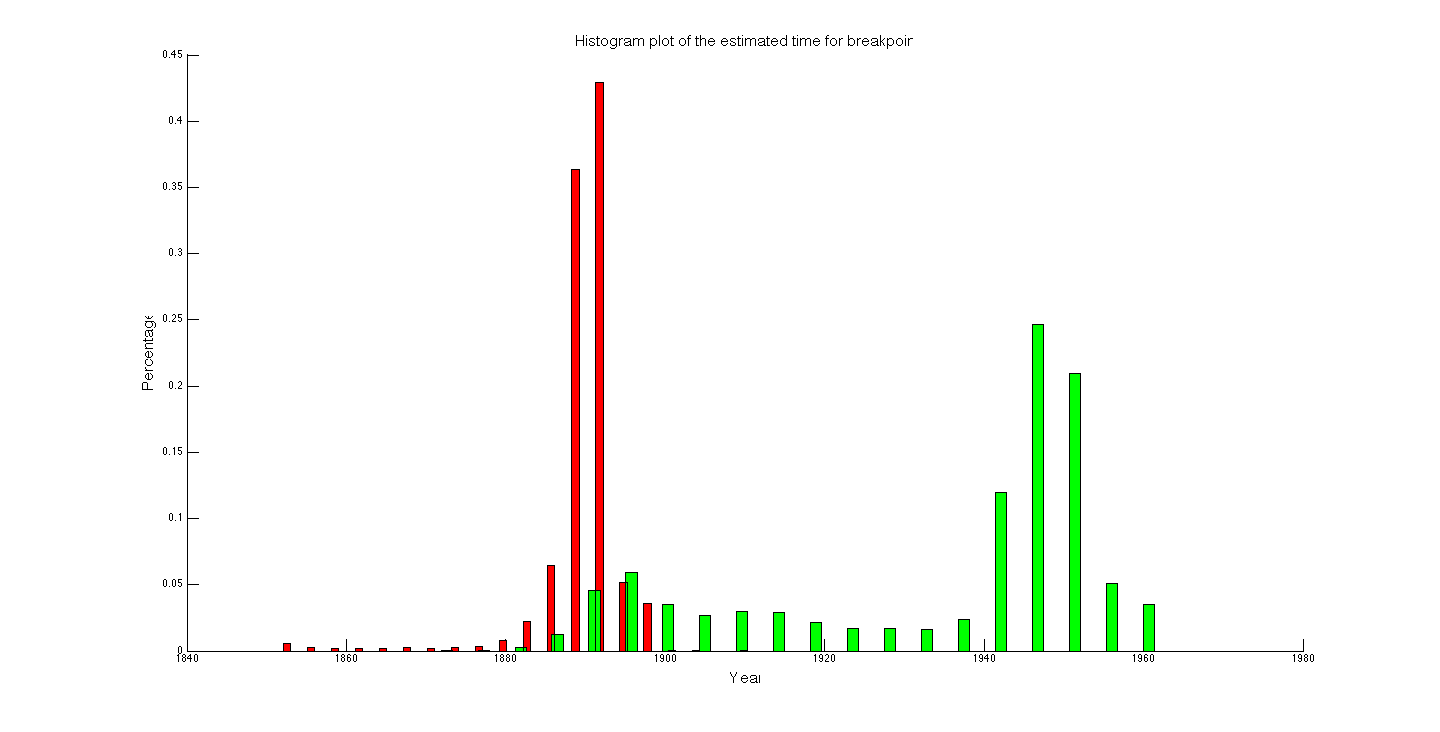
\includegraphics[scale=0.26]{./Figures/tpost2.png}
\caption{Histogram plot of the breakpoints.}
\label{fig:tpost2}
\end{figure}

As is seen in the above figure we have almost the same density as in figure \ref{fig:tpost1} for the first breakpoint, indicating a high accuracy of the results. Whereas we for the second breakpoint have rather large tails spanning almost the entire time period. This result is rather disappointing since we can expect to have a bad estimation of our second breakpoint. The samples that are drawn from the posterior are represented in figure \ref{fig:t2}.

\begin{figure}[H]
\centering
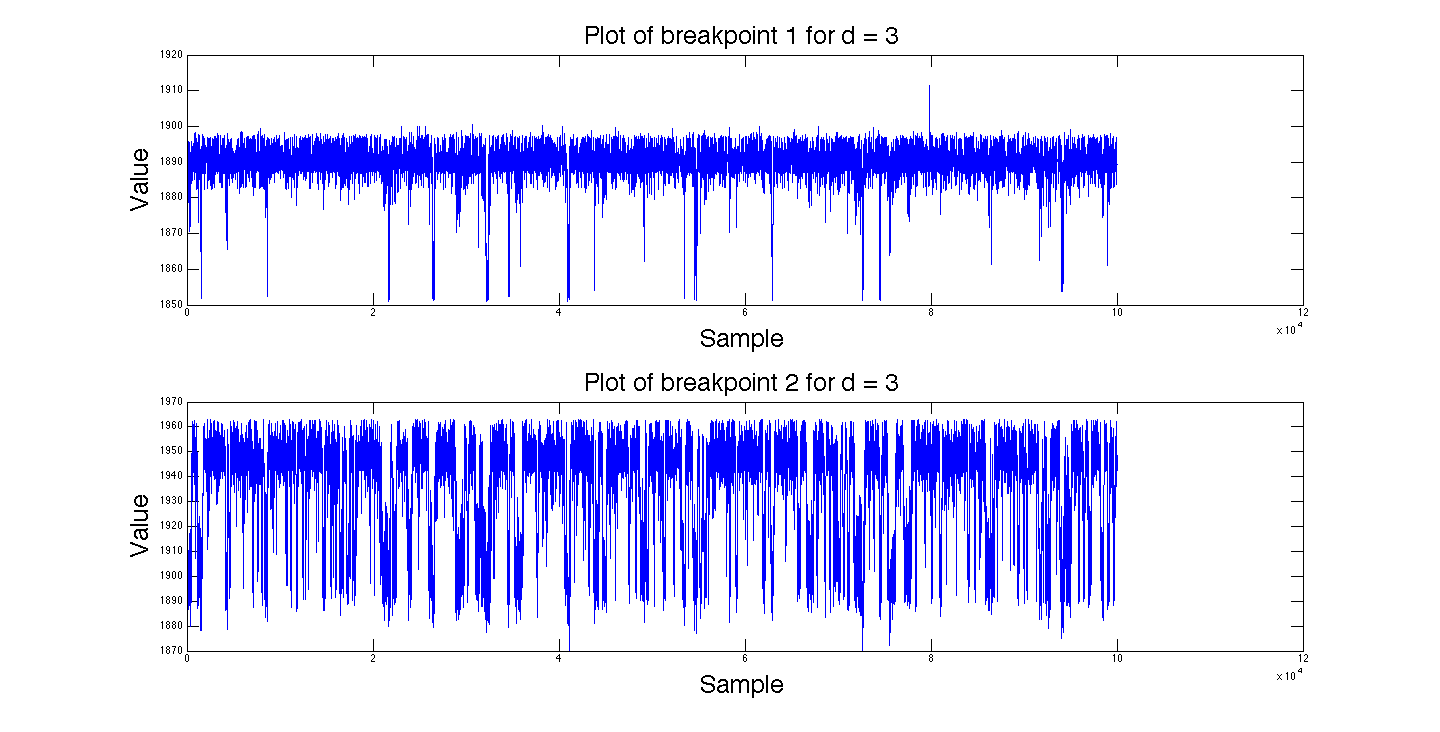
\includegraphics[scale=0.26]{./Figures/t2.png}
\caption{Visualization of the draws for both of the breakpoints.}
\label{fig:t2}
\end{figure}

As is seen in the figure above there is a small dependence of the draws, which could result in bad estimatations. \\
We turn our eyes toward the histograms of the intensties in figure \ref{fig:lpost2}.

\begin{figure}[H]
\centering
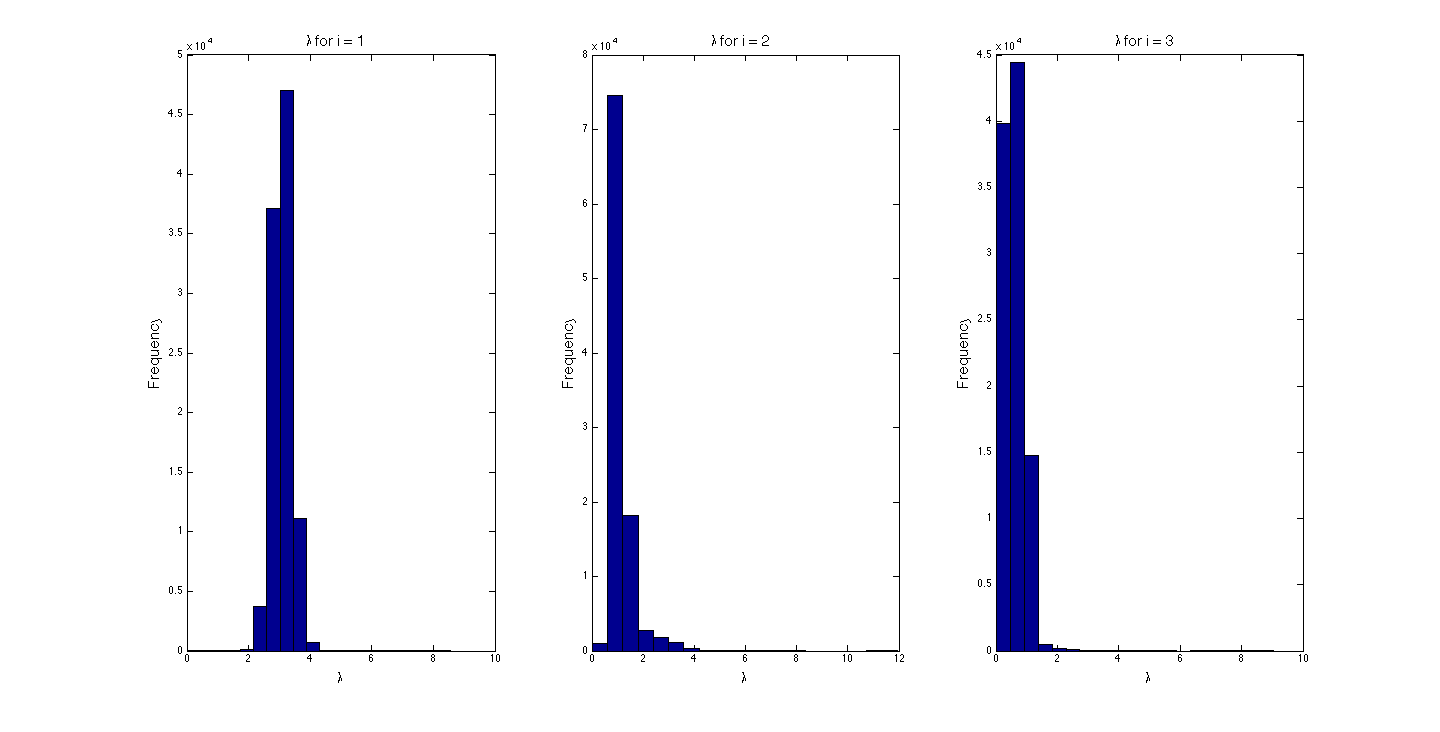
\includegraphics[scale=0.26]{./Figures/lpost2.png}
\caption{Histogram plot of the intensities.}
\label{fig:lpost2}
\end{figure}

By looking at the above figures we see that all of the intensities exhibit a $\Gamma$--distribution where they are centered around the values given by $\boldsymbol{\lambda} \approx (3.1,1.2,0.6)$. Since the first intensity and the first breakpoint are approximately the same as for one breakpoint we can assume that the "correct" breakpoint is somewhere between 1890--1891. \\ We finally look at the histogram of $\theta$ in figure \ref{fig:thetapost2}.

\begin{figure}[H]
\centering
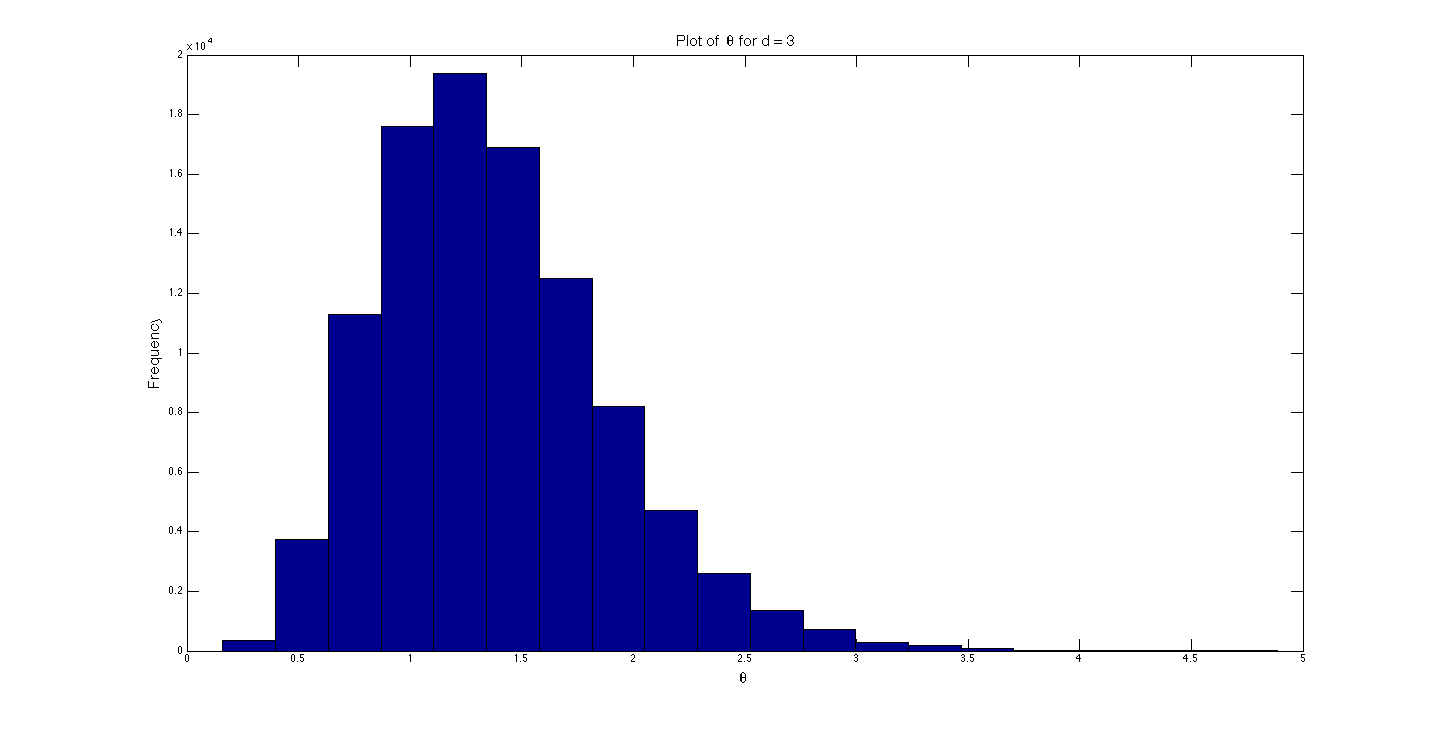
\includegraphics[scale=0.26]{./Figures/thetapost2.png}
\caption{Histogram plot of $\theta$.}
\label{fig:thetapost2}
\end{figure}

The histogram is highly indicative of $\Gamma$--distribution centered around $\approx 1.38$.

\newpage
\subsubsection*{Three breakpoints}
As in the previous sections we begin with investigating where the breakpoints are located, which is seen in figure \ref{fig:bp3}.

\begin{figure}[H]
\centering
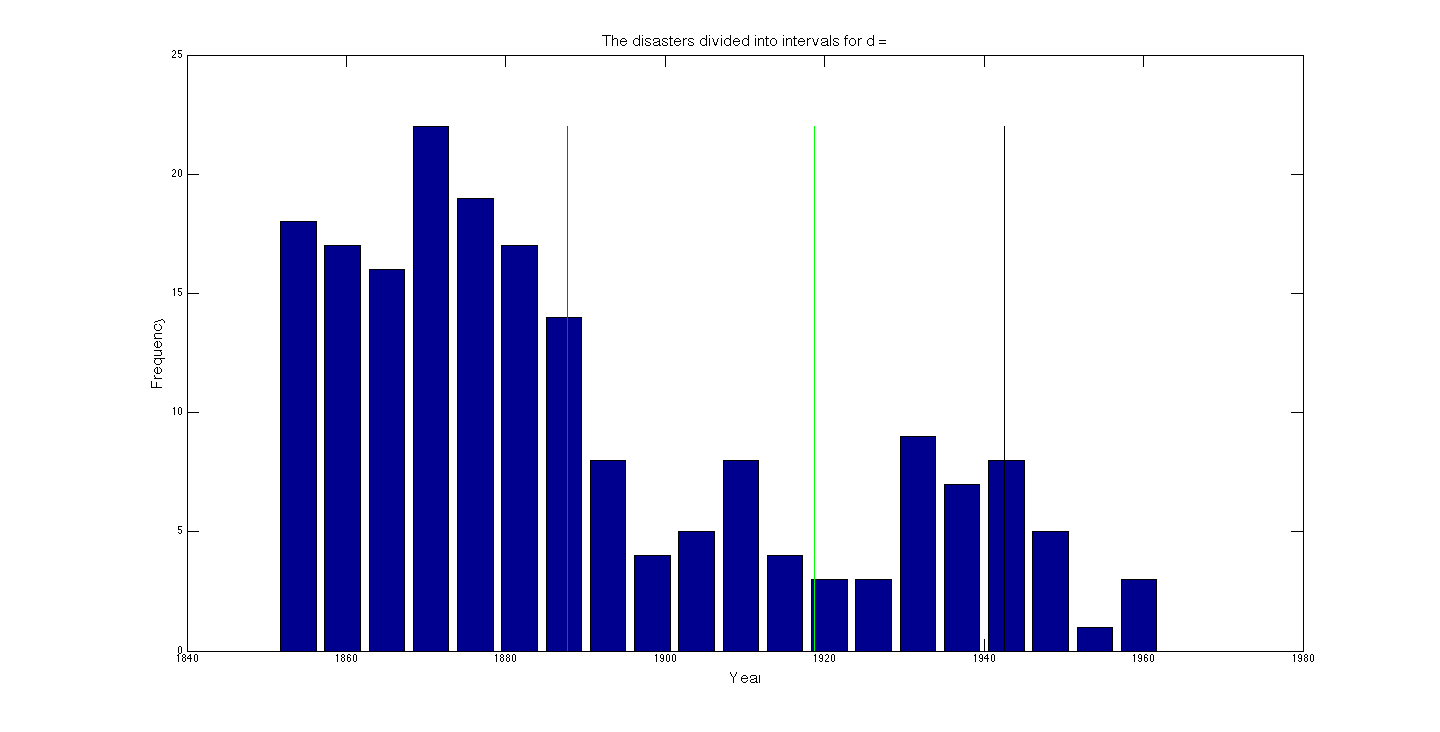
\includegraphics[scale=0.26]{./Figures/bp3.png}
\caption{Plot of where the breakpoints are located.}
\label{fig:bp3}
\end{figure}

From the above figure we see that the first breakpoint has moved to 1884 and the two other breakpoints are located around 1911 and 1942. It is difficult to comment on these locations since more than two breakpoints seem superflous. We thus look at the histogram plot of the breakpoints in figure \ref{fig:tpost3}.

\begin{figure}[H]
\centering
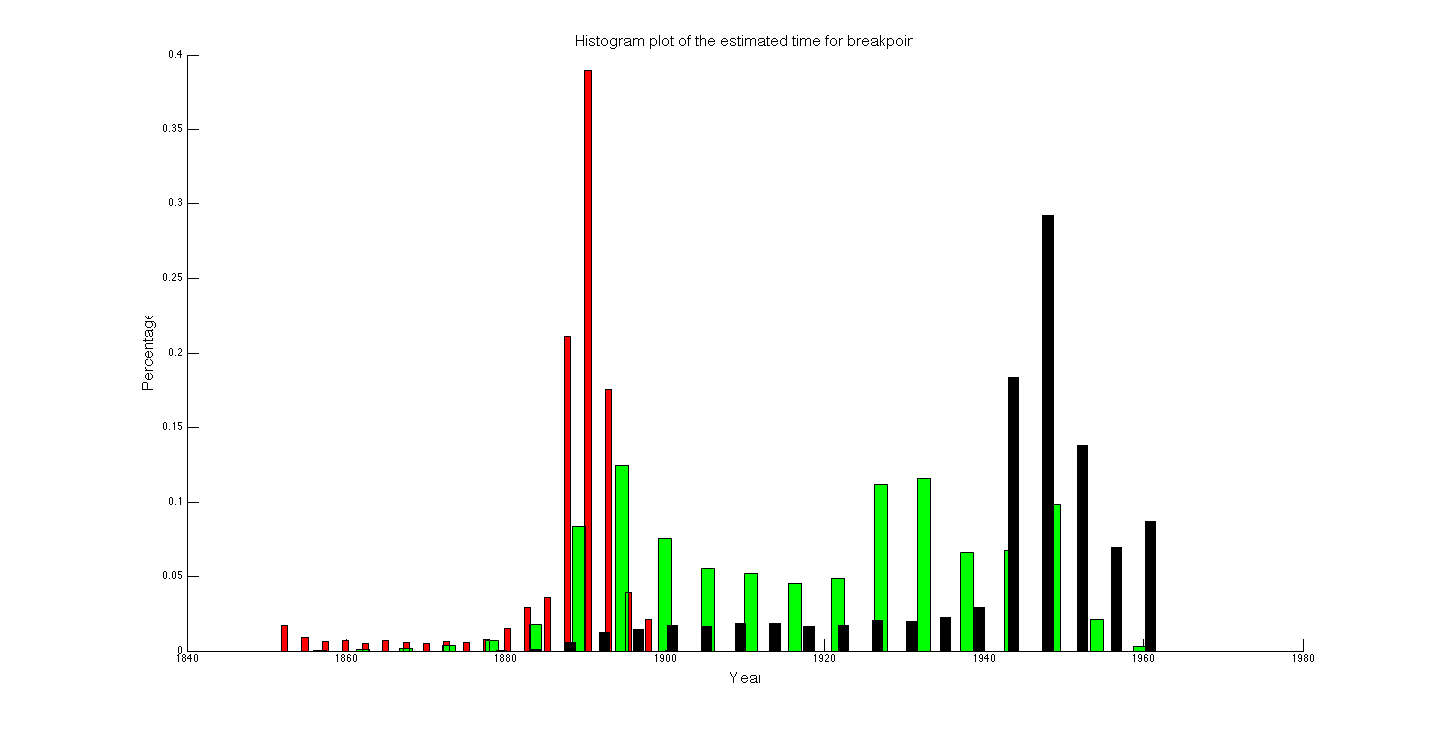
\includegraphics[scale=0.26]{./Figures/tpost3.png}
\caption{Histogram plot the breakpoints.}
\label{fig:tpost3}
\end{figure}

From the above figure we see that the histogram of the first breakpoint has a tiny tail to the left of the center suggesting a good estimation. The histogram of the second breakpoint is bad since we cannot distinguish a center of the density, which suggests that we will have a bad estimation in the breakpoint, it also spans over a large interval. The third histogram has almost the same density as that of the first density. It has a centered value with a small tail to the left, but most of the mass is located around the center. Here we can also note that it spans across a large interval. \\ We now investigate the behaviour of the draws from this posterior, which are visualized in figure \ref{fig:t3}.

\begin{figure}[H]
\centering
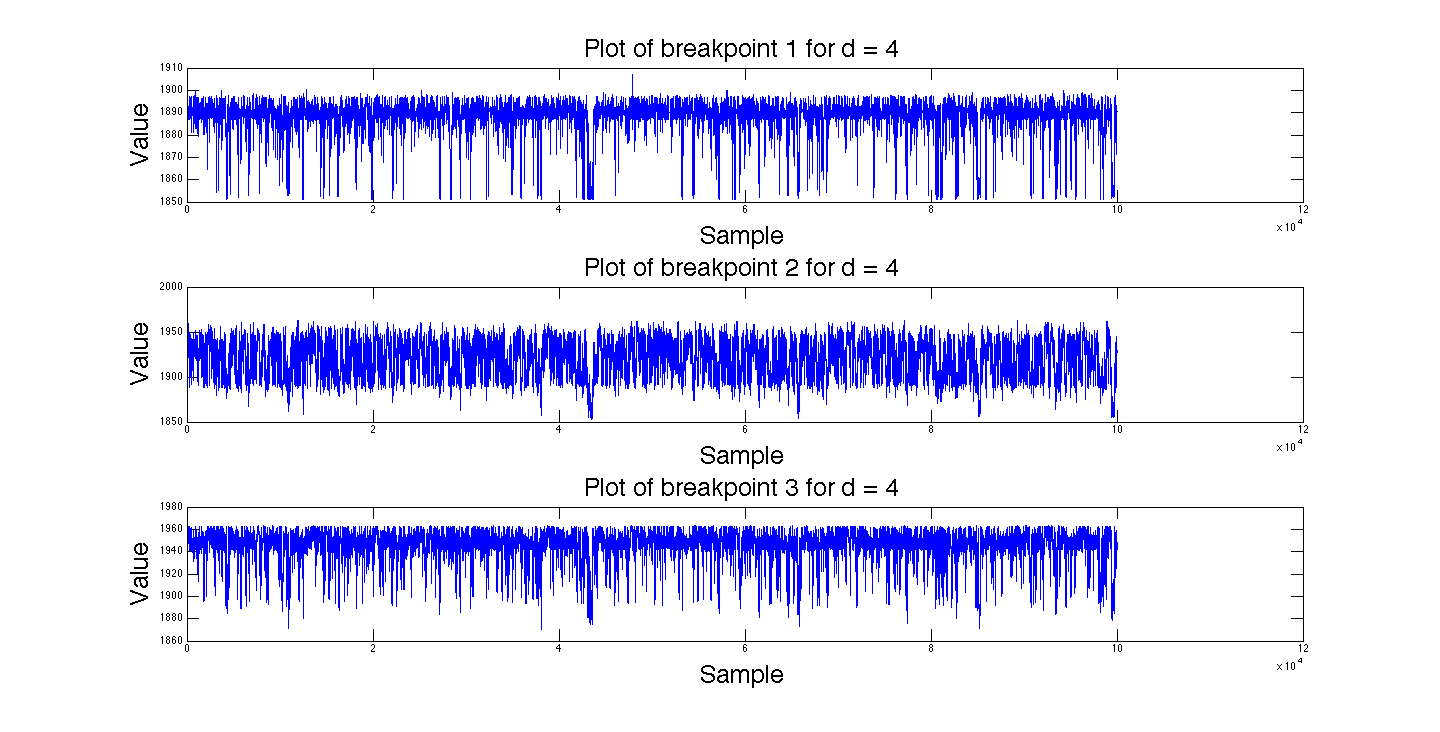
\includegraphics[scale=0.26]{./Figures/t3.png}
\caption{Visualization of the draws for both of the breakpoints.}
\label{fig:t3}
\end{figure}

As we can see in the above figure we have little dependence between the different draws. \\ We now move on to look at the histograms of the intensities.

\begin{figure}[H]
\centering
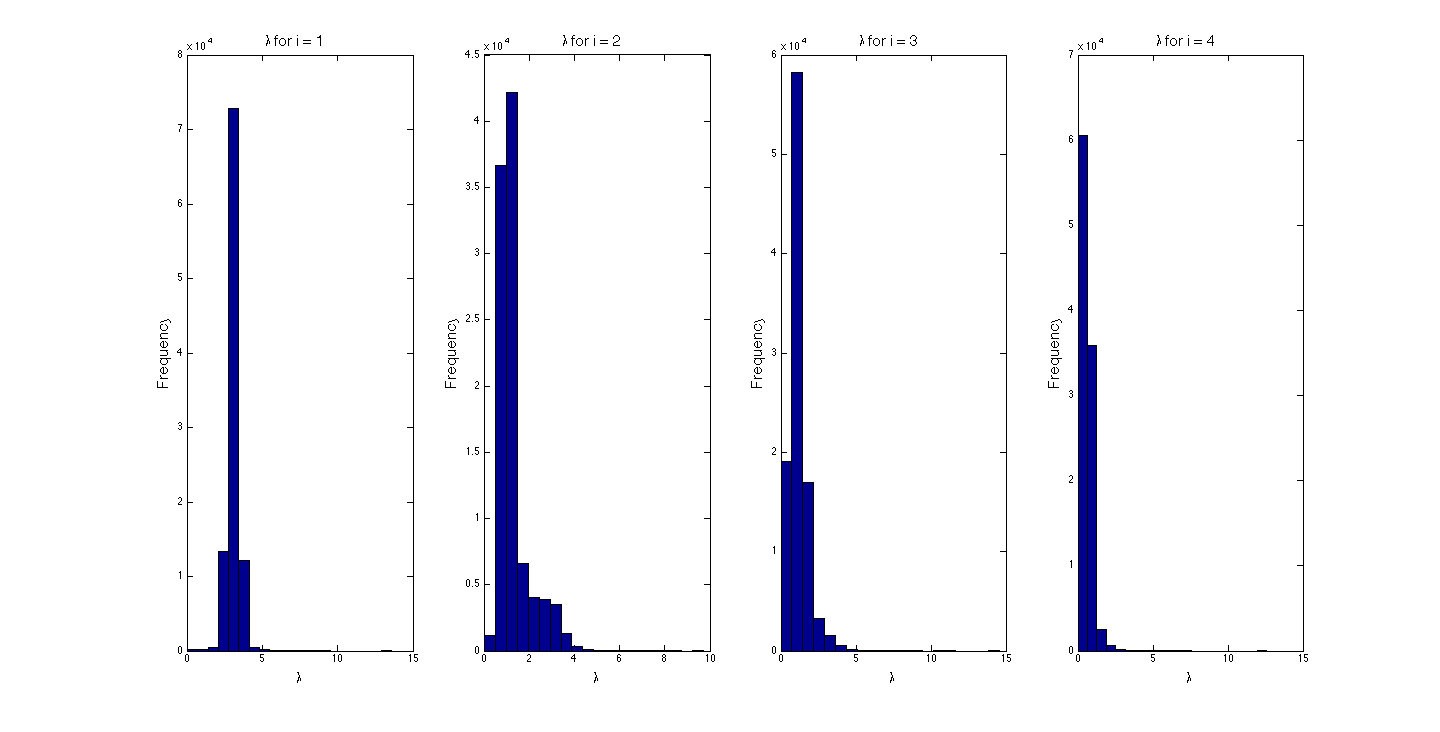
\includegraphics[scale=0.26]{./Figures/lpost3.png}
\caption{Histogram plots of the intensities.}
\label{fig:lpost3}
\end{figure}

From the above figure it is possible to discern a $\Gamma$--distribution for the distributions. The intensity for the first interval is still $\approx 3.1$. Lastly, we look at the histogram plot of $\theta$.

\begin{figure}[H]
\centering
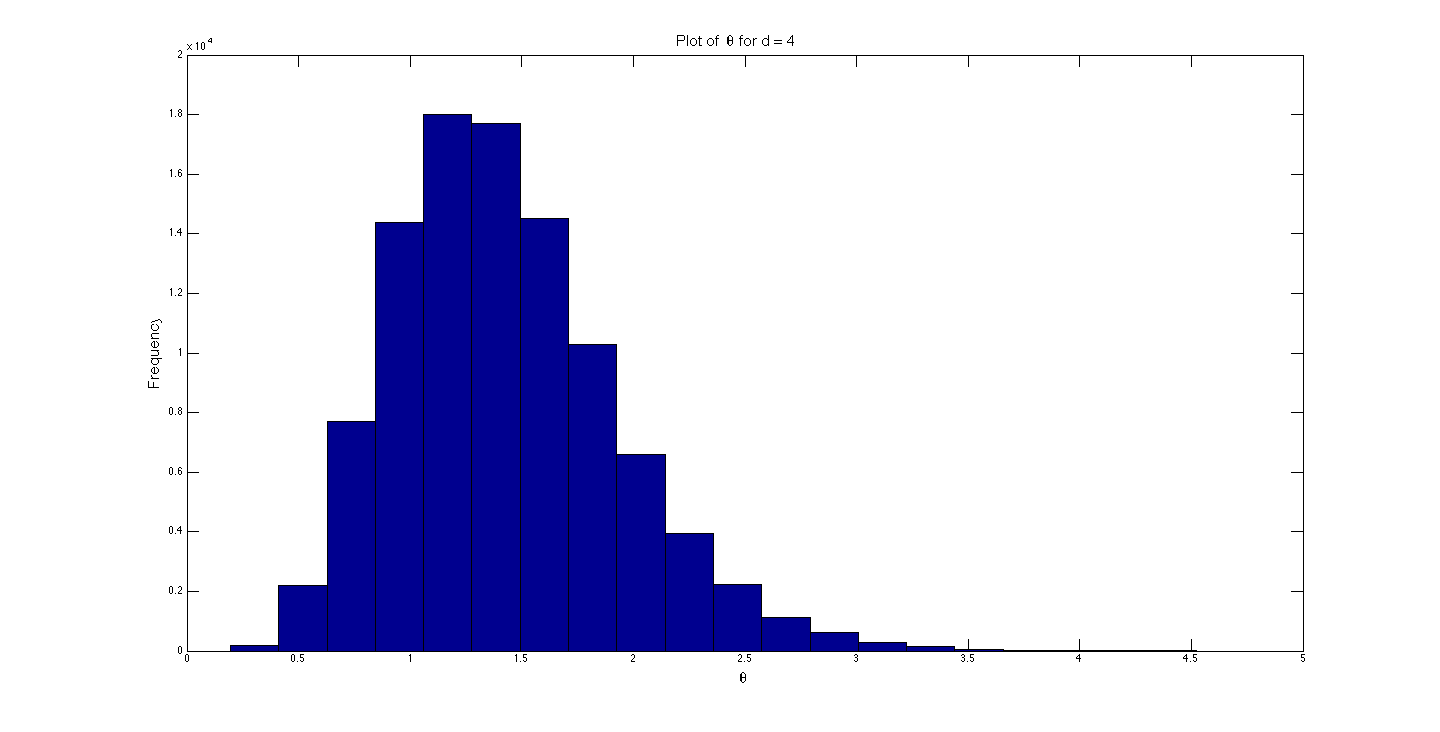
\includegraphics[scale=0.26]{./Figures/thetapost3.png}
\caption{Histogram plot of $\theta$.}
\label{fig:thetapost3}
\end{figure}

From the figure above, we see that $\theta$ still has the $\Gamma$--distribution but centered around 1.4.
\newpage
\subsubsection*{Four Breakpoints}

Finally, we investigate the behaviour using four breakpoints. We begin by looking at the location of the breakpoints as seen in figure \ref{fig:bp4}.

\begin{figure}[H]
\centering
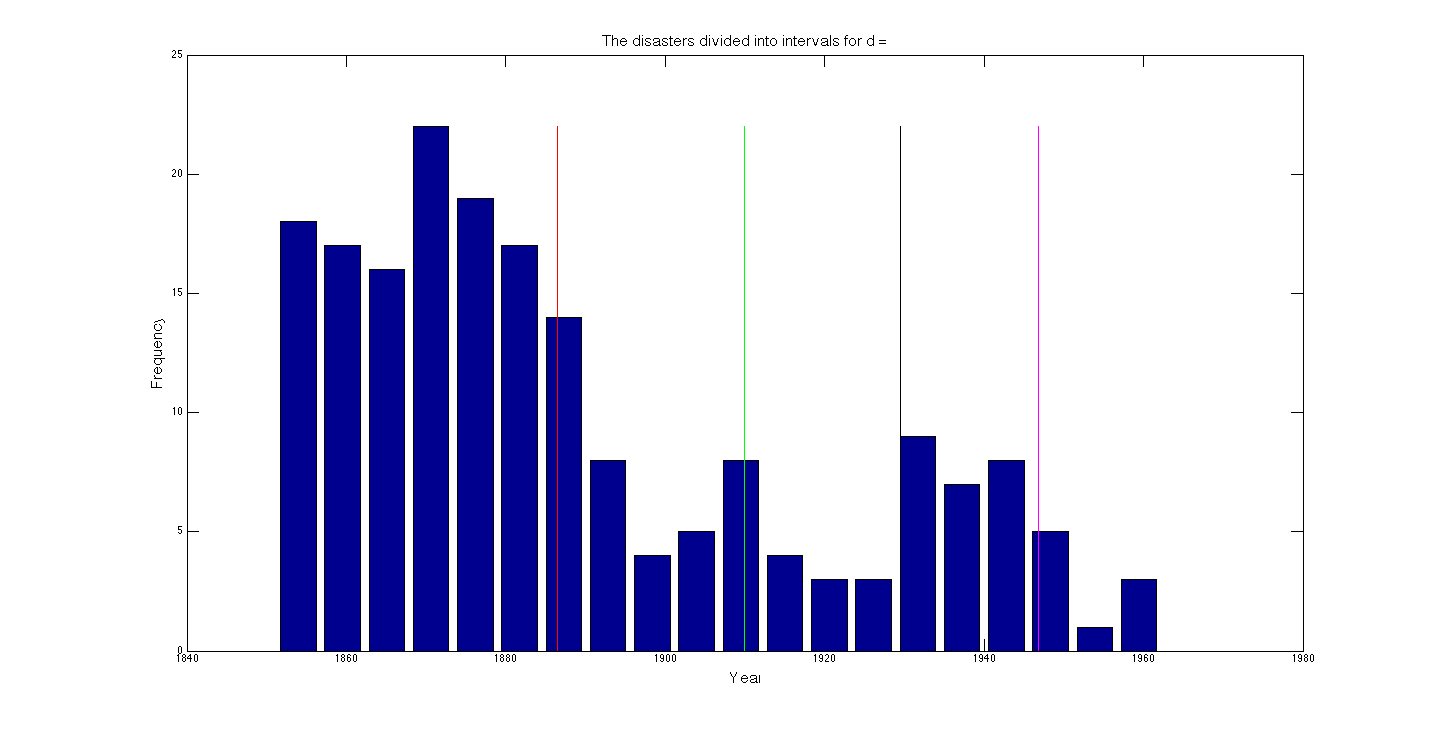
\includegraphics[scale=0.26]{./Figures/bp4.png}
\caption{Plot of where the breakpoints are located.}
\label{fig:bp4}
\end{figure}

From the above figure we see that the first breakpoint again has moved, but this time it did not move that far from the breakpoint suggested using only one breakpoint. It is now located around 1887. The second breakpoint is located around 1911, which is close to the second breakpoint when using three breakpoints. As in the previous section, it is difficult to say anything about the placement of the breakpoints since more than two seem superflous. We instead look at the histogram plot over the breakpoints.

\begin{figure}[H]
\centering
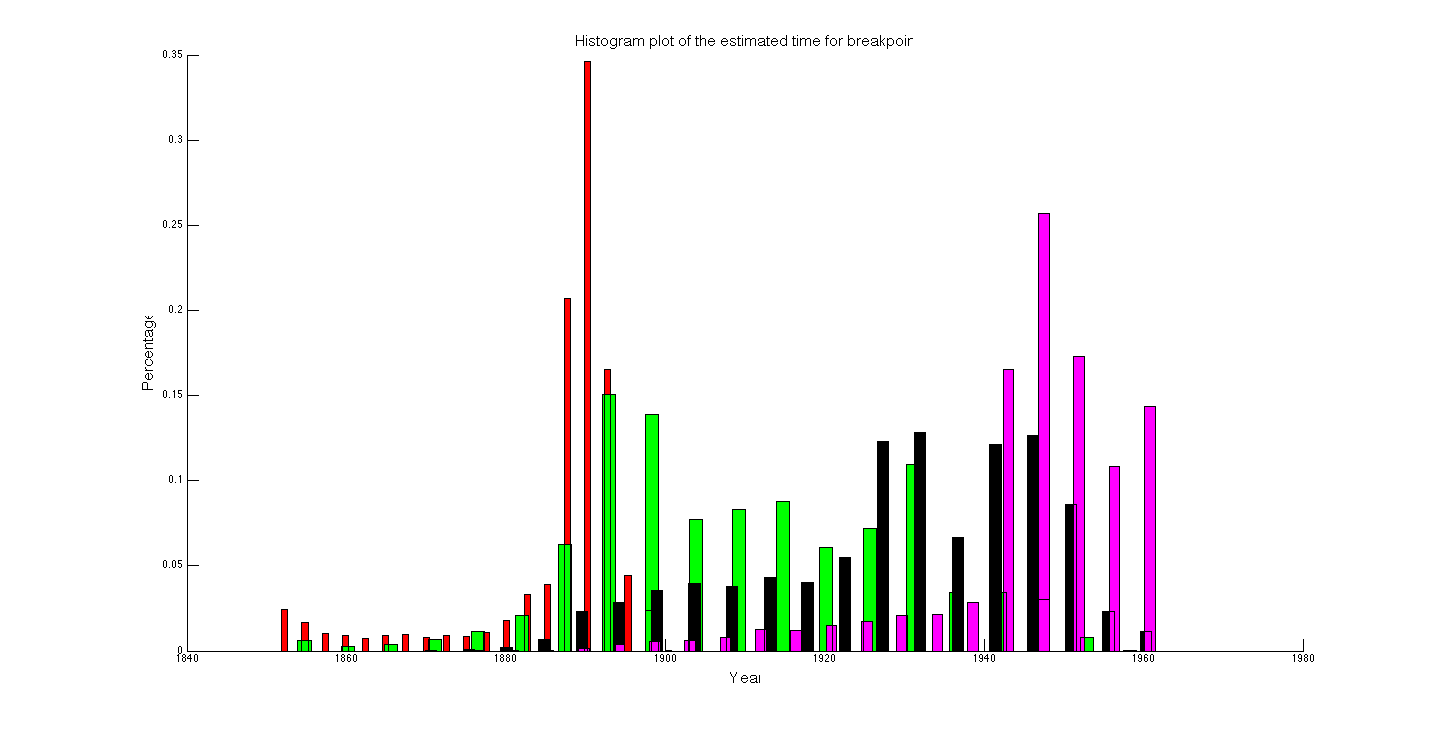
\includegraphics[scale=0.26]{./Figures/tpost4.png}
\caption{Histogram plot the breakpoints.}
\label{fig:tpost4}
\end{figure}

From the histogram above we can see that the first breakpoint behaves as previously around 1887. The second breakpoint also spans across a large interval, indicating a bad estimate. The third breakpoint has its mean around 1929, but spans across a large interval and is approximately uniform, indicating a bad estimate. The fourth breakpoint has its mean around 1948 and has almost the same distribution as the first, but with less frequency, here we can again conclude that this breakpoint could be good. We now move on to the draws of the breakpoints.

\begin{figure}[H]
\centering
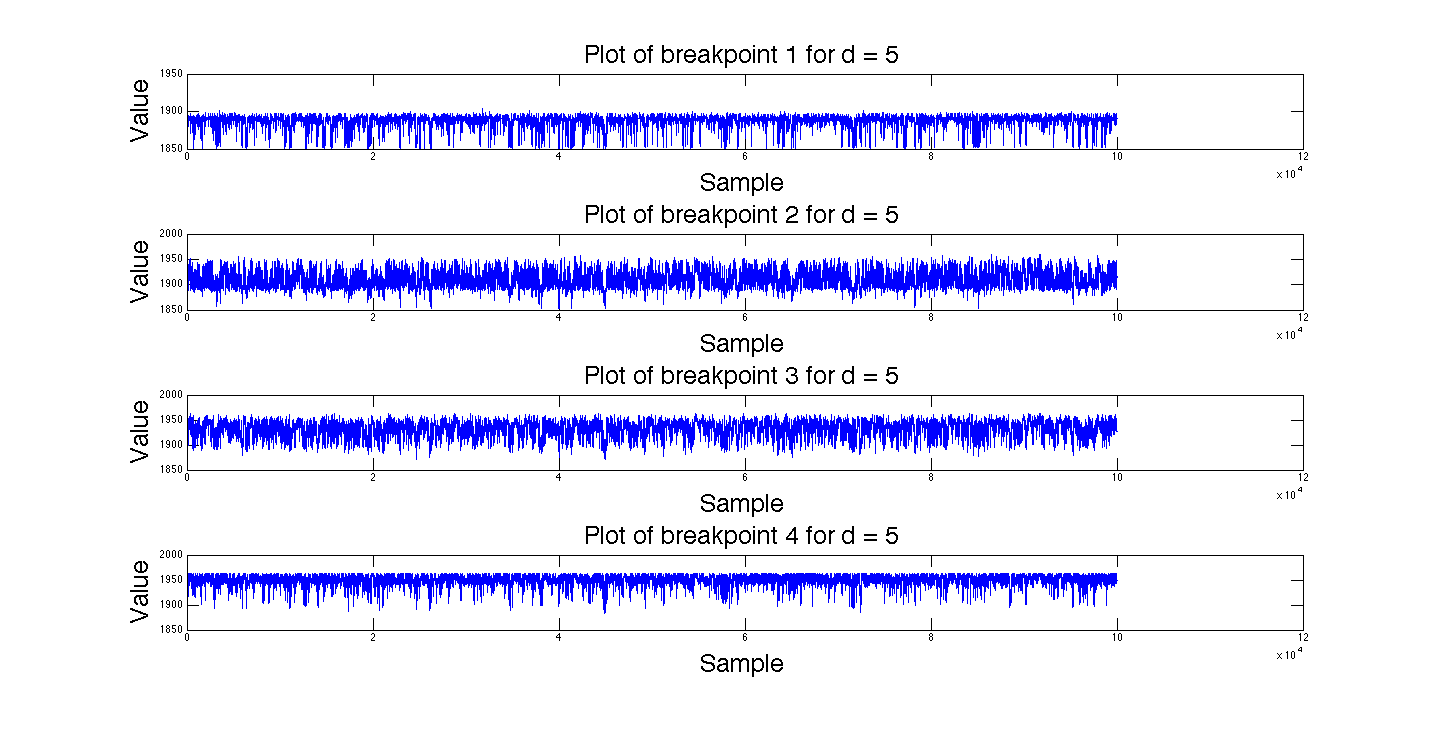
\includegraphics[scale=0.26]{./Figures/t4.png}
\caption{Visualization of the draws for both of the breakpoints.}
\label{fig:t4}
\end{figure}


As we can see in the above figure we have little dependence between the different drawshere as well. This indicates that our values of $\rho$ gives the draws a random behaviour.. \\ We now move on to look at the histograms of the intensities.

\begin{figure}[H]
\centering
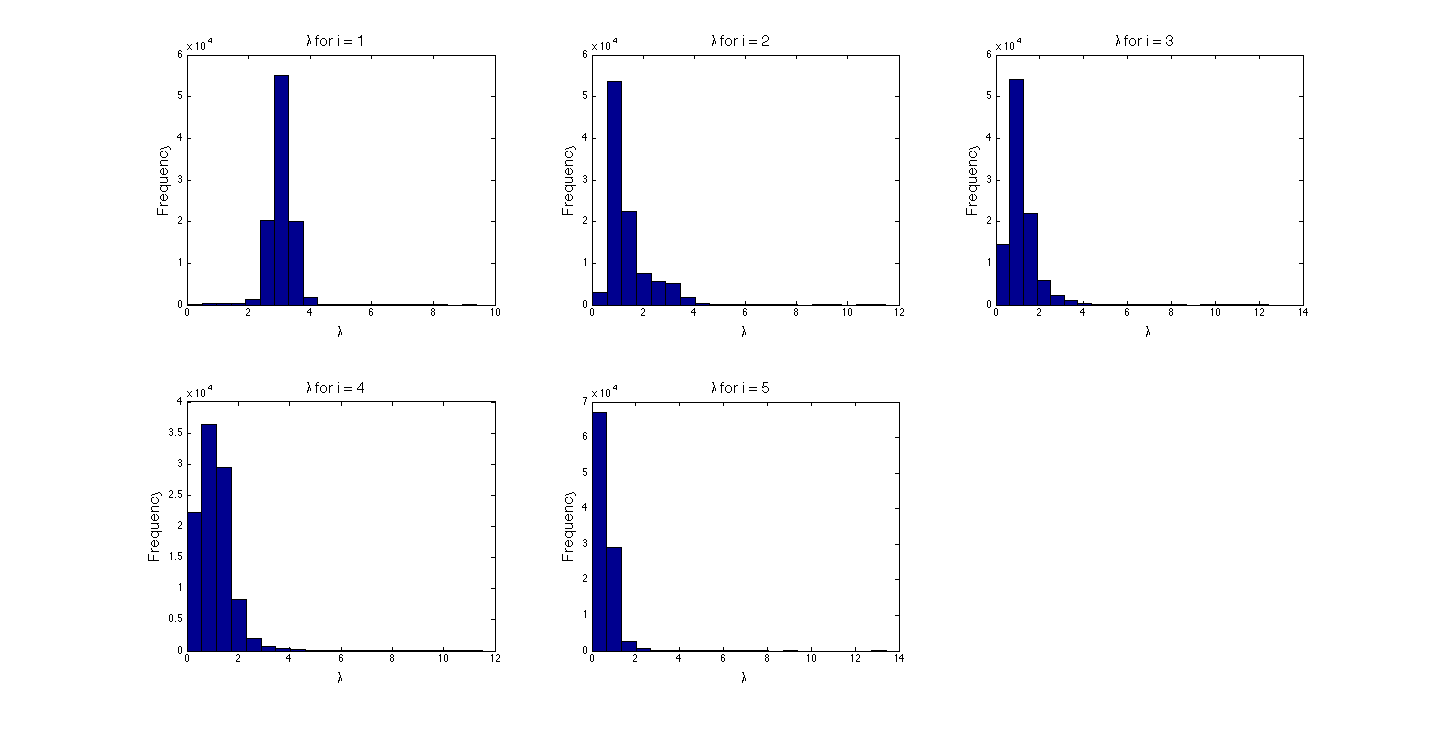
\includegraphics[scale=0.26]{./Figures/lpost4.png}
\caption{Histogram plots of the intensities.}
\label{fig:lpost4}
\end{figure}

From the above figure it is possible to discern a $\Gamma$--distribution for the distributions. The intensity for the first interval is still $\approx 3.1$. Lastly, we look at the histogram plot of $\theta$.

\begin{figure}[H]
\centering
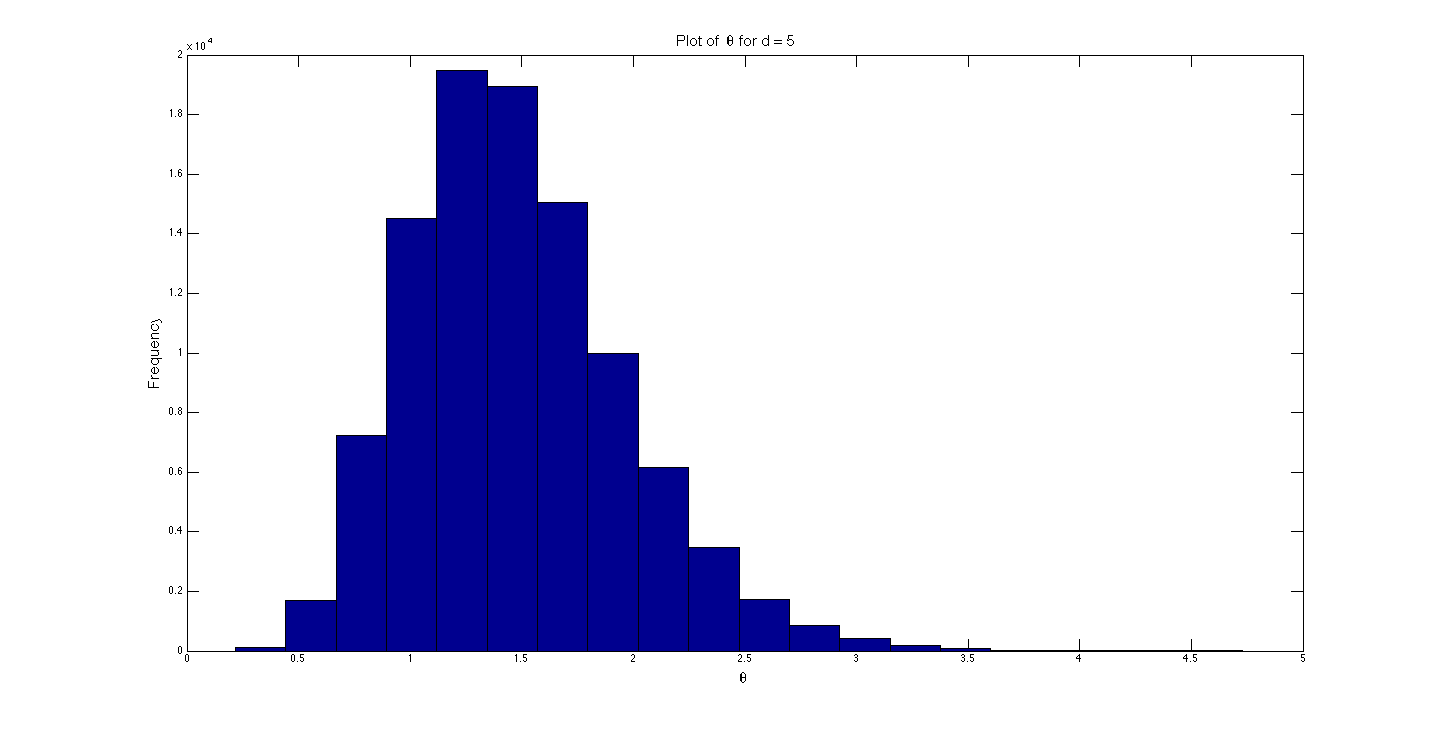
\includegraphics[scale=0.26]{./Figures/thetapost4.png}
\caption{Histogram plot of $\theta$.}
\label{fig:thetapost4}
\end{figure}

The histogram for $\theta$ is clearly has a $\Gamma$--distribution with center 1.46. \\ \\
We gather all of the breakpoints and intensities in table\ref{tablez} such as to get some overview, 


\begin{table}[H]
\begin{tabular}{|c|c|c|c|c|}
\hline
Breakpoints & 1 & 2 & 3 & 4 \\ \hline
$\boldsymbol{t}$ & 1891 & (1890,\:1937) & (1884,\:1911,\:1942) & (1889,\:1915,\:1933,\:1950) \\ \hline
$\boldsymbol{\lambda}$ & (3.1,\:0.9) & (3.1,\:1.2,\:0.6)  & (3.1,\:1.5,\:1.3,\:0.6)  & (3.1,\:1.3,\:1.1,\:1.2,\:0.6) \\ \hline
$\theta$ & 1.1995 & 1.3441 & 1.3536 & 1.408 \\ \hline
\end{tabular}
\label{tablez}
\end{table}

%These plots illustrate the expected breakpoints and therefore the associated intervals. As such we can evaluate if the interval data exhibit that of a gamma-distribution. We have illustrated the histograms in figures \ref{fig:tpost} of the $\boldsymbol{t}$-posteriors for each breakpoint, in order to investigate the probability of our breakpoint estimates. To also ensure that our prior $\theta$ has been established correctly, we here plot the histogram of $\theta$ indicating that it is of $\Gamma$-distributed character. The obtained $\theta$s and $\boldsymbol{\lambda}$ from our hyperprior is plotted in the figures \ref{fig:thetapost} and \ref{fig:lpost} respectively


%When sampling from the $f(\theta|\boldsymbol{\tau},\boldsymbol{\lambda},\boldsymbol{t})$ the histogram plot of the different $\theta$s. The same distribution occured for each case, as seen in the plots above. Hence we have only plotted two cases.
%Lambda posteriors


If the figures show a strong convergence towards an estimated value, we can assume that our approximation is good, i.e. when the histogram plots are localized around one value. Whenever a shift occurs we have a new Po-distribution in the data. Looking at the left figure in figure \ref{fig:bp2} we can easily see that the breakpoints is centered around 1891 with a small tail, thus indicating that the approximation is valid. By also looking at figure \ref{fig:bp1} we can easily see that there is a change in intensity at 1891. \\

When the data has been divided with two breakpoints, as seen in the right figure of figure \ref{fig:tpost2}. It is seen that the first breakpoint basically has the same distribution as only using one breakpoint, i.e. small tails and centered around 1891. However, the second breakpoint is centered around 1945 where most of the mass is allocated around this value. It is however also noted that there is a heavy tail of the distribution spanning across 50 years. \\

The left figure of figure \ref{fig:tpost3} shows the histograms of the three breakpoints. It is seen the the first breakpoint corresponds to almost the same previous values, i.e. centered around 1890, but one can note that there is a tail to the left. The second breakpoint is the most interesting, since there seems to be two centers, one in 1890 and one in 1940. Indicating an uncertainty in the estimation as the Monte Carlo approximation will be highly affected. The third breakpoint has the same distribution as the first and is centered around 1944. \\

\subsubsection*{Summary}
From the previous analysis we can deduce that if we would divide the disasters into blocks with different intensities, we would use one breakpoint at the year 1891. Giving the intensities of the disasters as the figures show in \ref{fig:lpost1}. The intensity between the years 1851--1891 would be $\lambda_1 \approx 3.1$ disasters per year and the intensity between 1891--1963 would be $\lambda \approx 0.9$. It can also be concluded that the chosen values for $\rho$ give a random and independent behaviour of the draws for the kernel of the MH algorithm. 
